\documentclass{article}

% Language setting
% Replace `english' with e.g. `spanish' to change the document language
\usepackage[english]{babel}

% Set page size and margins
% Replace `letterpaper' with `a4paper' for UK/EU standard size
\usepackage[letterpaper,top=2cm,bottom=2cm,left=3cm,right=3cm,marginparwidth=1.75cm]{geometry}
\usepackage{CJKutf8}
% Useful packages
\usepackage{amsmath}
\usepackage{graphicx}
\usepackage{setspace}
\usepackage{float}
\usepackage{subfigure}
\usepackage{array}
\usepackage[section]{placeins}
\usepackage[colorlinks=true, allcolors=blue]{hyperref}
\usepackage[export]{adjustbox}

\author{B10209040 陳彥倫}

\begin{document}
\thispagestyle{empty}
\hfill {\scshape \large Cloud Physics, Fall 2023 } \hfill {\scshape P1}
\smallskip
\hrule
\begin{CJK*}{UTF8}{bsmi}
\bigskip
\bigskip
\bigskip

\centerline{\huge \textbf {HW4}}
\bigskip
\centerline{\textbf {B10209040 陳彥倫}}

\section*{1. Radar}

\subsection*{(1)}
    \begin{large}
        Plot results:
        \begin{figure}[!htbp]
            \centering
            \subfigure[i = -3]{
            \begin{minipage}[t]{0.5\linewidth}
            \centering
            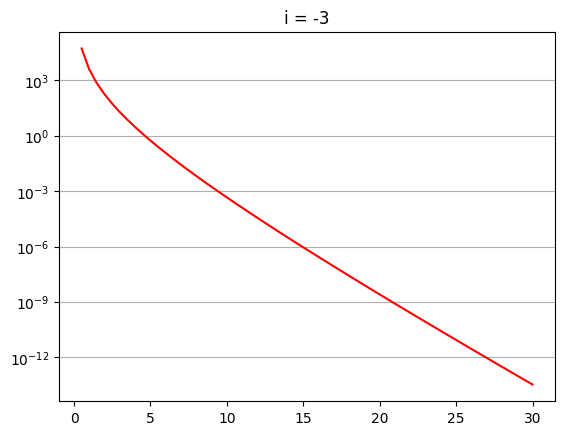
\includegraphics[scale=0.4]{output.png}
            %\caption{fig1}
            \end{minipage}%
            }%
            \subfigure[i = 0]{
            \begin{minipage}[t]{0.5\linewidth}
            \centering
            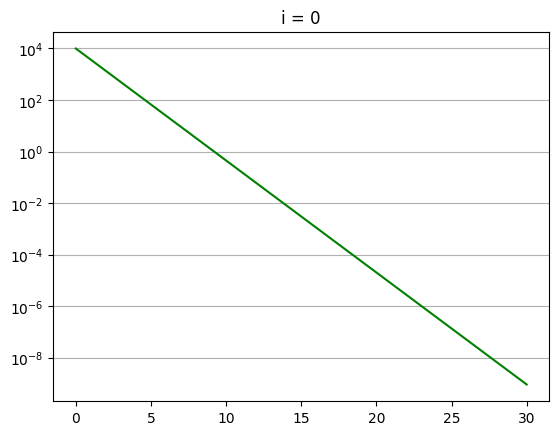
\includegraphics[scale=0.4]{output2.png}
            %\caption{fig2}
            \end{minipage}%
            }%

            \subfigure[i = 3]{
            \begin{minipage}[t]{0.5\linewidth}
            \centering
            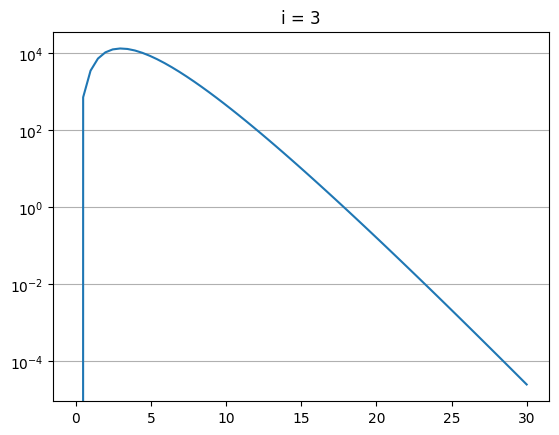
\includegraphics[scale=0.4]{output3.png}
            %\caption{fig2}
            \end{minipage}%
            }%
        \end{figure}
    \end{large}

\subsection*{(2)}
    \begin{large}
        \begin{center}
            \begin{displaymath}
                Z \equiv \sum\limits_{V}D^6 = \int_{0}^{\infty} D^6n(D) \,dD = \int_{0}^{\infty} D^6 \cdot N_0 \cdot D^i \cdot exp(-\lambda D^j) \,dD
            \end{displaymath}
        \end{center}

        \bigskip

        若$i = -3$時,將上述式子積分可得解析解:
            \begin{displaymath}
                Z = -10^4(D^3 + 3D^2 + 6D + 6)e^{-D}\bigg|^{\infty}_{0} = \mathbf{6 \times 10^4}
            \end{displaymath}

        \newpage

        若$i = 0$:
        \begin{displaymath}
            Z = -10^4(D^6 + 6D^5 + 30D^4 + 120D^3 + 360D^2 + 720D +720)e^{-D}\bigg|^{\infty}_{0} = \mathbf{7.2 \times 10^6}
        \end{displaymath}

        若$i = 3$:
        \begin{displaymath}
            Z = -10^4(D^9 + 9D^8 + 72D^7 + 504D^6 + \dots + 362880D + 362880)e^{-D}\bigg|^{\infty}_{0} = \mathbf{3.6288 \times 10^9}
        \end{displaymath}

    \end{large}

\subsection*{(3)}
    \begin{large}
        
    
    \end{large}


\begin{spacing}{2}
    \begin{large}
        \: \\
        \textbf{Approach:} \\
        為求水滴從雲底墜落至地表所花時間,利用終端速度與顆粒半徑大小等關係式\\
        $\frac{dZ}{dt} = -u(R) + W$計算。然而在只有在雲中水滴會受到上升氣流之影響,因此將此處$W = 0$代入。
        半徑的遞迴計算以Mason equation求得。\\
        \textbf{Discussion:} \\
        由結果可以看出初始半徑較小的粒子到達地面所花費的時間較長,成長之半徑大小的比例亦較大。落至地面之最終半徑
        大小較預期的為小,可能與單位的設定與公式計算有關。

        
        

        
    \end{large}
\end{spacing}

\end{CJK*}
\end{document}